\subsubsection{Zur Frage der Vollständigkeit des Werkverzeichnisses}

Die 24 Lücken (grau markiert) in dem 63 Opusnummern umfassenden Werk von
Högn machen eines deutlich: Es sind nicht alle Kompositionen erhalten.
An dieser Stelle sollte deshalb neben den Gründen, für den Verlust
einiger seiner Kompositionen besonders die Fragen nach Anzahl und Art
der nicht erhaltenen Kompositionen in den Mittelpunkt gestellt werden.

Der Hauptgrund für das Abhandenkommen einiger von Högns Kompositionen
liegt an den unzureichenden Vorkehrungen zum dauerhaften Erhalt seines
kompositorischen Nachlasses. Nach Högns Tod hatte die Haushälterin Rosa
Beischmied den Auftrag erhalten, sich um die Auflösung seiner Wohnung
zu kümmern. \footnote{Interview Nr. 20, Gertraud von Molo, 23.11.2004,
Absatz 35; Interview Nr. 2, Barbara Essigmann, 27.12.2002, Absatz 76}
Da sämtliche Kompositionen in Ruhmannsfelden verblieben, lag es an der
Haushälterin, ihren weiteren Verwendungszweck zu bestimmen. Allein
schon die vielen verschiedenen Fundorte von Högns Kompositionen
sprechen dafür, dass Beischmied an mehrere Personen beziehungsweise
Institutionen die noch in Högns Wohnung verbliebenen Werke
weitergegeben hatte. Die Fundorte waren im Einzelnen: der Notenschrank
und Dachboden des linken Seitenschiffs der Pfarrkirche St. Laurentius,
der Pfarrhof St. Laurentius, die Wohnung des ehemaligen
Kirchenchorleiters und Leiters des Ruhmannsfeldener Männerchors Franz
Danziger, das Haus der Sängerin Mathilde Glasschröder sowie die
Bayerische Staatsbibliothek, München.

\begin{figure}
\img{}
\caption{}
\end{figure}


\begin{supertabular}{m{3.7419999cm}m{0.8cm}m{4.3cm}m{2.3009999cm}m{4.801cm}}
{\centering   [Warning: Image ignored]
% Unhandled or unsupported graphics:
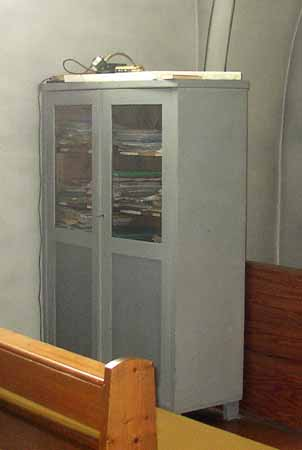
\includegraphics[width=3.674cm,height=5.509cm]{pictures/zulassungsarbeit-img062.jpg}
 \par}
Notenschrank der Pfarrkirche St.
Laurentius &

\begin{figure}
\img{}
\caption{}
\end{figure}

\multicolumn{2}{m{5.3cm}}{{\raggedleft   [Warning: Image ignored]
% Unhandled or unsupported graphics:
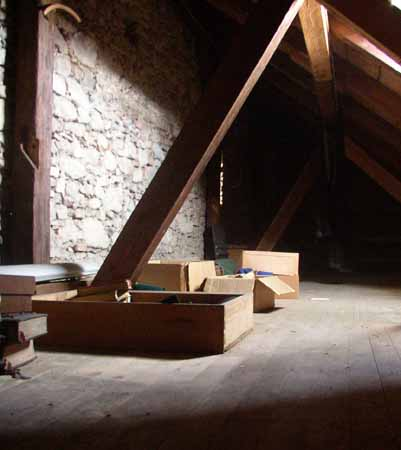
\includegraphics[width=4.951cm,height=5.509cm]{pictures/zulassungsarbeit-img063.jpg}
 \par}
Dachboden des linken Seitenschiffs der
Pfarrkirche St. Laurentius} &

\begin{figure}
\img{}
\caption{}
\end{figure}
\multicolumn{2}{m{7.302cm}}{  [Warning: Image ignored]
% Unhandled or unsupported graphics:
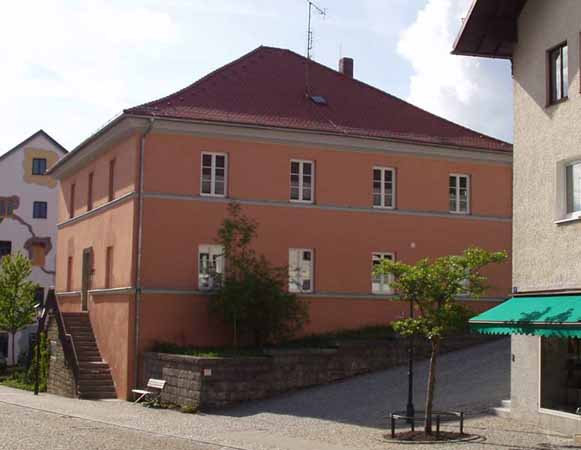
\includegraphics[width=7.091cm,height=5.509cm]{pictures/zulassungsarbeit-img064.jpg}

Pfarrhof St. Laurentius,
Ruhmannsfelden}\\

\begin{figure}
\img{}
\caption{}
\end{figure}
\multicolumn{2}{m{4.742cm}}{  [Warning: Image ignored]
% Unhandled or unsupported graphics:
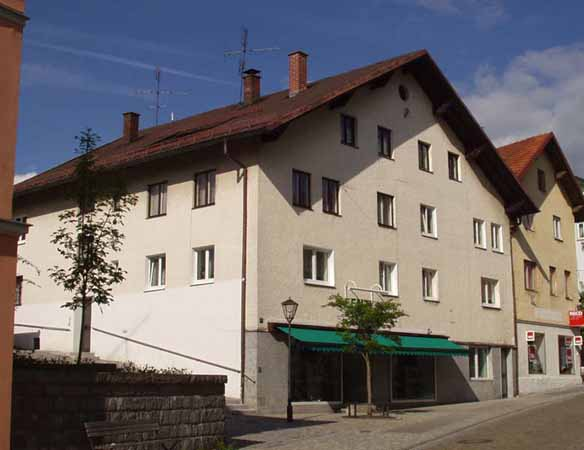
\includegraphics[width=4.531cm,height=3.493cm]{pictures/zulassungsarbeit-img065.jpg}

Wohnung von Franz Danziger} &

\begin{figure}
\img{}
\caption{}
\end{figure}
\multicolumn{2}{m{6.801cm}}{  [Warning: Image ignored]
% Unhandled or unsupported graphics:
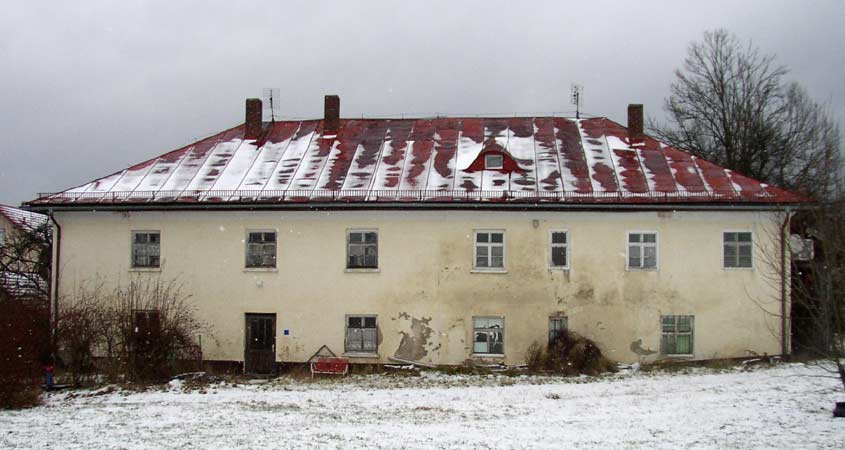
\includegraphics[width=6.549cm,height=3.487cm]{pictures/zulassungsarbeit-img066.jpg}

\begin{figure}
\img{}
\caption{}
\end{figure}

Haus der Sängerin Mathilde
Glasschröder} &

\begin{figure}
\img{}
\caption{}
\end{figure}

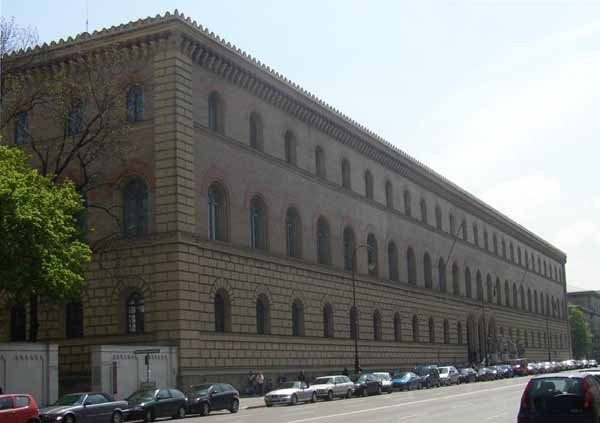
\includegraphics[width=4.509cm,height=3.491cm]{pictures/zulassungsarbeit-img067.jpg}

Bayerische Staatsbibliothek

\begin{figure}
\img{}
\caption{}
\end{figure}

Einzeln verstreute, über den ganzen Ort Ruhmannsfelden aufgewahrte Werke
unterliegen weit mehr der Vernichtungsgefahr aus Unwissenheit, als der
in einem Archiv aufbewahrte Bestand des Nachlasses. Es ist daher nicht
verwunderlich, dass es konkrete Anhaltspunkte gibt, wonach
Kompositionen von Högn vernichtet worden sein könnten. Da Franz
Danziger nicht nur Kirchenchorleiter, sondern zur Zeit der Auflösung
von Högns Wohnung auch Leiter des Ruhmannsfeldener Männerchores war und
im Turnverein-Orchester unter Högn mitwirkte, \footnote{Dokument Nr.
56, Auszug aus den Memoiren von Franz Danziger sen., 1984} müsste seine
Wohnung ein weit ergiebigerer Fundort gewesen sein. Hier war aber kein
einziges weltliches Werk neben den entdeckten geistlichen Kompositionen
zum Vorschein gekommen. Der Sohn des ehemaligen Kirchenchorleiters
räumte in seinem Brief vom 25.10.2002 ein, dass seine Mutter bei
Entsorgungsarbeiten eventuell auch Werke von Högn vernichtet haben
könnte. \footnote{Korrespondenz Nr. 7, Brief von Franz Danziger an
Josef Friedrich, 25.10.2002} Es ist anzunehmen, dass selbst zu Högns
Lebzeiten einige seiner Werke eventuell verloren gegangen sind. Nach
der Entlassung von Högn als Chorregent durch Reicheneder haben die
Sängerinnen Barbara Essigmann und Mathilde Glasschröder alle
Kompositionen aus der Kirche mitgenommen und in Högns Wohnung getragen.
Die Haushälterin Rosa Beischmied trug sie kurz darauf wieder
zurück. \footnote{Interview Nr. 2, Barbara Essigmann, 27.12.2002,
Absatz 56} Dass bei diesem „Gezerre“ um die Noten nach Högns Entlassung
das eine oder andere Werk verloren ging, liegt durchaus im Bereich des
Möglichen. Nach Aussage von Barbara Essigmann hat die Sängerin Maria
Schröck weit mehr Kompositionen von Högn als nur die „Josephi“-Messe
ihrem neuem Chorregenten Fritz Goller in Deggendorf (siehe
 „„Josephi“-Messe F-Dur op. 62“, Seite
) übergeben. \footnote{Interview Nr. 2,
Barbara Essigmann, 27.12.2002, Absatz 18} Höchstwahrscheinlich sind
einige von Högns Kompositionen in Deggendorf verloren gegangen, denn
weder im Nachlass von Fritz Goller \footnote{Korrespondenz Nr. 27,
E-Mail von Martina Goller an Josef Friedrich, 4.3.2003} noch in den
Notenbeständen seiner ehemaligen Wirkungsstätten Mariä
Himmelfahrt \footnote{Korrespondenz Nr. 32, E-Mail von Hermann Wellner
an Josef Friedrich, 25.3.2003} und St. Martin konnten Werke von Högn
ausfindig gemacht werden. Da nicht bekannt ist, an wie viele Personen
Rosa Beischmied Kompositionen übergeben hat, ist nicht auszuschließen,
dass noch weitere seiner Werke existieren. Ihr Aufbewahrungsort bleibt
jedoch unbekannt. Weitere mögliche Fundorte wurden deshalb ohne einen
konkreten Hinweis erfolglos. Nachforschungen über den Verbleib von
Kompositionen beim Achslacher Männerchor, den Franz Danziger bis ins
hohe Rentenalter leitete und mit dem er 1983 ein Marienlied von Högn
aufführte, \footnote{Dokument Nr. 74, Zeitungsartikel aus dem
Viechtacher Bayerwald-Boten, 1983} brachten keine positiven
Ergebnisse. \footnote{Korrespondenz Nr. 85, E-Mail von Franz Aichinger
an Josef Friedrich, 4.1.2005} Centa Schwannberger, die Ehefrau von
Rudolf Schwannberger, der zusammen mit Högn die Sängerriege des
Turnvereins leitete, hat den Notenbestand ihres Mannes den
Geißkopfsängern übergeben. Hier verlaufen sich die Spuren.\footnote{
Korrespondenz Nr. 91, Telefonat von Helmut Gärtner an Josef Friedrich,
8.1.2005} Auch die Nachfahren von Vitus Voit, einem Mitwirkenden im
Turnverein-Orchester, konnten keine von Högns Kompositionen finden.

Es stellt sich nun die Frage nach der Anzahl der nicht mehr erhaltenen
Kompositionen von Högn. Da Högns Opuszahlen nur eine sehr
eingeschränkte Aussagekraft in Bezug auf die tatsächlich komponierten
Werke haben (siehe  „Anmerkungen zu den
Opuszahlen“, Seite ) und Högn selbst kein
Werkverzeichnis hinterließ, kann keine genaue Zahl verlorener
Kompositionen genannt werden. Das Verhältnis von 24 fehlenden
Opuszahlen zu 50 erhaltenen Werken (39 Werke mit Opuszahl + 4 Werke mit
doppelter Opuszahl + 7 Werke ohne Opuszahl), suggeriert in etwa ein
Verhältnis von 1 zu 2. Demnach kann man die Meinung vertreten, dass
ungefähr zwei Drittel von Högns ursprünglichem Werk erhalten sind.

Einige konkrete Hinweise lassen Rückschlüsse zu, wie sich der unbekannte
Teil seines Werks zusammengesetzt haben könnte. Nur von einer
verschollenen Komposition ist der Namen bekannt. Drei Briefe erwähnen
eine „Herz-Jesu-Litanei.“ Es muss eine bedeutende Komposition gewesen
sein, denn Högn wollte sie sogar drucken lassen.
\footnote{Dokument Nr. 60, Brief von Sebaldus-Verlag, Bamberg an August Högn, 20.5.1947;
Dokument Nr. 59, Brief von Gregorius-Verlag, Regensburg an August Högn, 9.6.1947;
Dokument Nr. 57, Brief von Gregorius-Verlag, Regensburg an August Högn, 16.6.1947}
In Otto
Geyers Buch „Schule und Lehrer in Niederbayern“ ist ein Kapitel den
niederbayerischen Lehrerkomponisten gewidmet. Als eine Gattung von
Högns Werk erwähnt Geyer hier auch Requien. \footnote{Geyer, Seite 95}
Das Libera e-moll op. 50 ist wohl der klägliche Rest von Högns
Requien-Schaffen. Einige Hinweise lassen Rückschlüsse auf Högns
verschollene weltliche Kompositionen zu. An seinem 80. Geburtstag
versprach Högn dem Ruhmannsfeldener Männerchor unter der Leitung von
Franz Danziger \zitat{„weiteres Notenmaterial zur Verfügung
zu stellen.“ } \footnote{Dokument Nr. 49, Zeitungsartikel aus
Viechtacher Bayerwald-Bote, 5.8.1958} Laut Johann Glasschröder, dem
damaligen Vorstand, hat Högn für den Männerchor tatsächlich
komponiert. \footnote{Interview Nr. 24, Johann Glasschröder,
28.12.2004, Absatz 32} Högn hatte neben dem Ruhmannsfeldener Männerchor
noch zu weiteren Männerchören Kontakt. Bei der 1919 gegründeten
Sängerriege des Turnvereins Ruhmannsfelden unter der Leitung von Rudolf
Schwannberger fungierte Högn sogar zeitweise als Dirigent.\footnote{
Dokument Nr. 104, Protokoll der Turnvereinsversammlung, 27.9.1919;
Dokument Nr. 105, Protokoll der Turnvereinsversammlung, 29.12.1919} Das
Marienlied Nr. 9 op. 34 ist eine Auftragskomposition für einen
Männerchor aus Regen. Högn hatte zum Leiter dieses Regener Chores ein
freundschaftliches Verhältnis, wie aus dem im sehr kameradschaftlichen
Ton gehalten Brief an Högn ersichtlich ist. \footnote{Dokument Nr. 62,
Brief von „Franzl“, Regen an August Högn, 17.6.1928} Diese Männerchöre
könnten Gelegenheiten zur Aufführung und daher Anlass zur Entstehung
von Kompositionen geboten haben.

\begin{flushleft}
\tablefirsthead{}
\tablehead{}
\tabletail{}
\tablelasttail{}
\begin{supertabular}{m{2.809cm}}

\begin{center}

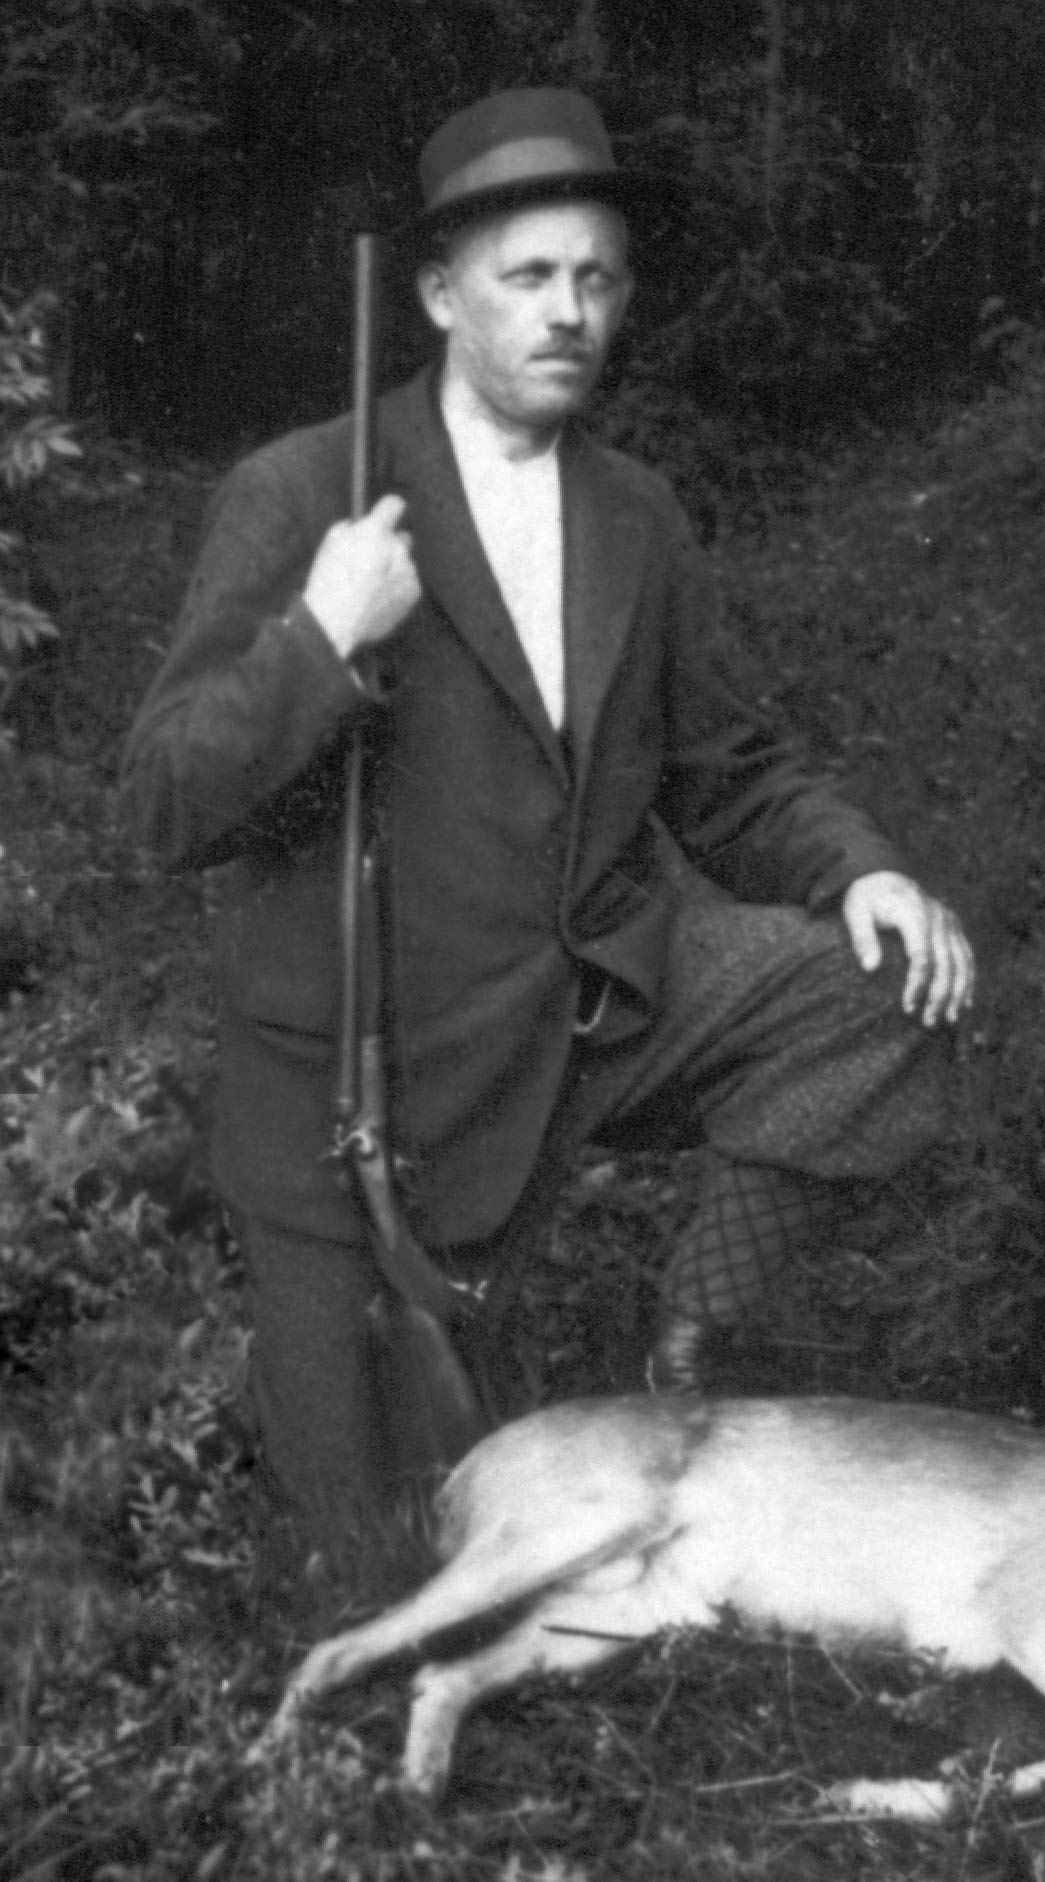
\includegraphics[width=2.626cm,height=4.68cm]{pictures/zulassungsarbeit-img068.jpg}

\end{center}
August Högn auf der Jagd\\
\end{supertabular}
\end{flushleft}

\begin{figure}
\img{}
\caption{}
\end{figure}

Nach Barbara Essigmann lassen sich auch diese weltlichen Chorsätze
thematisch näher bestimmen. Högn, ein begeisterter Jäger, soll viele
„Jägerlieder“ geschrieben haben, die beispielsweise auf einer
Geburtstagsfeier des Kreisjägermeisters und Kirchenchormitgliedes
Rudolf Schwannberger oder in der Schule gesungen wurden.\footnote{
Interview Nr. 5, Barbara Essigmann, 2.1.2003, Absatz 40} Das Fach
Singen in der Schule kann als weiteres kompositorisches Betätigungsfeld
von August Högn angesehen werden. Wenn er nicht eigene Lieder schrieb,
dann fertigte er mit Sicherheit Arrangements für seine Schüler und
Schülerinnen an. \footnote{Interview Nr. 16, Maria Freisinger,
25.8.2004, Absatz 24} Der Satz des Adventliedes „Tauet Himmel“ ist ein
Beispiel dafür. Auf das Notenblatt dieses Arrangements vermerkte Högn:
„Aus meinen Kinderliedern.“ Högn hatte sich anscheinend eine Sammlung
von Liedsätzen für den Schuleinsatz angelegt. Wenn es sich bei diesen
Schulliedern um eine ähnliche Zusammenstellung handelte, wie die
Sammlung der Marienlieder und Grablieder, dann ist davon auszugehen,
dass neben Abschriften und Arrangements auch eigene Kompositionen dazu
gehörten. Högn hat über 30 Marienlieder und 7 Grablieder
zusammengestellt und durchnummeriert. Die ersten 12 Nummern der
Marienlieder und die ersten 4 Nummern der Grablieder stellen eigene
Kompositionen dar, dann folgen Arrangements und Abschriften. Ob Högn
noch mehr an Instrumentalmusik als nur den im Selbstverlag erschienenen
Marsch „In Treue fest!“ hinterlassen hat, darüber kann spekuliert
werden. Normalerweise schreibt ein Komponist mehrere Stücke zu einem
bestimmten Genre, bis er dann das ausgereifteste Werk in Druck gibt.
Und ermuntert nicht eine erschienene Komposition zu weiterer
Kompositionsarbeit am gleichen Genre? Es wäre ebenfalls denkbar, dass
Kompositionen auch für die Orchesterriege des Turnvereins
Ruhmannsfelden entstanden sind, die Högn in den 20er- und 30er-Jahren
des 20. Jahrhunderts leitete.
